\section{Rule-Based Classification}

\begin{frame}{Using \uppercase{if-then} Rules for Classification}
  \begin{itemize}
  \item \textbf{Represent the knowledge in the form of {\color{airforceblue}IF-THEN rules}.}
    \begin{itemize}
    \item E.g., if \texttt{age} $\leq 30$ AND \texttt{student} = "yes" THEN buys\_computer = "yes".
    \item Readable.
    \end{itemize}
  \item \textbf{Rule {\color{airforceblue}antecedent/precondition} vs. rule {\color{airforceblue}consequent}}.
  \item \textbf{Assessment of a rule R: coverage and accuracy.}
    \begin{itemize}
    \item $n_{\text{covers}} = \#$ of tuples covered by $R$ (antecedent if true).
    \item $n_{\text{correct}} = \#$ of tuples correctly classified by $R$.
    \item $\text{coverage}(R) = \frac{n_{\text{covers}}}{|D|}$ with $D$ training data set.
    \item $\text{accuracy}(R) = \frac{n_{\text{correct}}}{n_{\text{covers}}}$.
    \end{itemize}
  \end{itemize}
\end{frame}

\begin{frame}{Using \uppercase{if-then} Rules for Classification (II)}
  \begin{itemize}
  \item \textbf{If more than one rule are triggered, need {\color{airforceblue}conflict resolution}.}
    \begin{itemize}
    \item \textbf{\color{airforceblue}Size ordering:}
      \begin{itemize}
      \item Assign the highest priority to the triggered rule that has the "toughest" requirement \\ (i.e., the most attribute tests).
      \end{itemize}
    \item \textbf{\color{airforceblue}Class-based ordering:}
      \begin{itemize}
      \item Decreasing order of prevalence or misclassification cost per class.
      \end{itemize}
    \item \textbf{\color{airforceblue}Rule-based ordering} (decision list):
      \begin{itemize}
      \item Rules are organized into one long priority list,\\
        according to some measure of rule quality, or by experts.
      \end{itemize}
    \end{itemize}
  \end{itemize}
\end{frame}

\begin{frame}{Rule Extraction from a Decision Tree}
  \begin{itemize}
  \item \textbf{Rules are {\color{airforceblue}easier to understand} than large trees.}
  \item \textbf{Rule can be created for {\color{airforceblue}each path from the root to a leaf.}}
    \begin{itemize}
    \item The leaf holds the class prediction.
    \end{itemize}
  \item \textbf{Each attribute-value pair along the path forms a conjunction:}
  \end{itemize}
  \begin{columns}
    \begin{column}{0.45\textwidth}
      \vspace{-3.3cm}
      \begin{itemize}
      \item \textbf{Example:}
        \begin{itemize}
        \item IF \texttt{age} $\leq$ 30 AND \texttt{student} = "no" \\
          THEN \texttt{buys\_computer} = "no".
        \item IF \texttt{age} $\leq$ 30 AND \texttt{student} = "yes" \\
          THEN \texttt{buys\_computer} = "yes".
        \item IF \texttt{age} $31\ldots40$ THEN \texttt{buys\_computer} = "yes".
        \item
        \item
        \end{itemize}
      \end{itemize}
    \end{column}
    \begin{column}{0.55\textwidth}
      \centering
      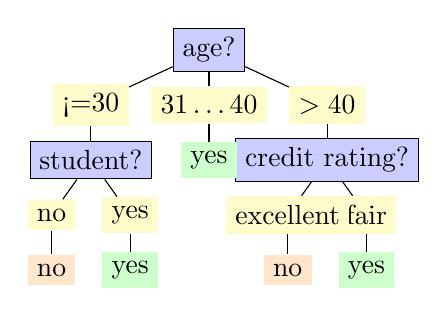
\begin{tikzpicture}
        \node[draw, fill=blue!20] at (0,0) (a) {age?};
        \node[fill=yellow!20] at (-1.5,-0.7) (b) {<=30};
        \node[fill=yellow!20] at (0,-0.7) (c) {$31\ldots40$};
        \node[fill=yellow!20] at (1.5,-0.7) (d) {$>40$};
        \node[draw, fill=blue!20] at (-1.5,-1.4) (e) {student?};
        \node[fill=yellow!20] at (-2,-2.1) (eno1) {no};
        \node[fill=yellow!20] at (-1,-2.1) (eyes1) {yes};
        \node[fill=orange!20] at (-2,-2.8) (eno2) {no};
        \node[fill=green!20] at (-1,-2.8) (eyes2) {yes};
        \node[draw, fill=blue!20] at (1.5,-1.4) (g) {credit rating?};
        \node[fill=yellow!20] at (2,-2.1) (gf) {fair};
        \node[fill=yellow!20] at (1,-2.1) (gex) {excellent};
        \node[fill=orange!20] at (1,-2.8) (gno) {no};
        \node[fill=green!20] at (2,-2.8) (gyes) {yes};
        \node[fill=green!20] at (0,-1.4) (f) {yes};

        \draw (a)--(b);
        \draw (a)--(c);
        \draw (a)--(d);
        \draw (b)--(e);
        \draw (c)--(f);
        \draw (d)--(g);
        \draw (e)--(eno1);
        \draw (e)--(eyes1);
        \draw (eno1)--(eno2);
        \draw (eyes1)--(eyes2);
        \draw (g)--(gex);
        \draw (g)--(gf);
        \draw (gex)--(gno);
        \draw (gf)--(gyes);
      \end{tikzpicture}
    \end{column}
  \end{columns}
\end{frame}

\begin{frame}{Rule Induction: Sequential Covering Method}
  \begin{itemize}
  \item \textbf{Sequential covering algorithm:}
    \begin{itemize}
    \item Extracts rules directly from training data.
    \end{itemize}
  \item \textbf{Typical sequential covering algorithms:}
    \begin{itemize}
    \item FOIL, AQ, CN2, RIPPER.
    \end{itemize}
  \item \textbf{Rules are learned {\color{airforceblue}sequentially}.}
    \begin{itemize}
    \item Each rule for a given class $C_i$ will cover many tuples of $C_i$, but none (or few) of the tuples of other classes.
    \end{itemize}
  \item \textbf{Steps:}
    \begin{itemize}
    \item Rules are learned one at a time.
    \item Each time a rule is learned, the tuples covered by the rule are removed.
    \item The process repeats on the remaining tuples unless termination condition, e.g., when no more training examples left or when the quality of a rule returned is below a user-specified threshold.
    \end{itemize}
  \item \textbf{Compare with decision-tree induction:}
    \begin{itemize}
    \item That was learning a set of rules simultaneously.
    \end{itemize}
  \end{itemize}
\end{frame}

\begin{frame}{Sequential Covering Algorithm}
  \begin{itemize}
  \item \textbf{While (enough target tuples left):}
    \begin{itemize}
    \item generate a rule;
    \item remove positive target tuples satisfying this rule;
    \end{itemize}
    \centering
    \begin{tikzpicture}
      \draw[fill=airforceblue] (0,0) ellipse (5.2 and 2.5) (0,0) node [text=black] {};
      \draw[fill=white] (0,1) ellipse (2 and 1.2) (0,0) node [text=black] {};
      \draw[fill=white] (-3,-0.2) ellipse (2 and 1.2) (0,0) node [text=black] {};
      \draw[fill=white] (3,0) ellipse (2 and 1.2) (0,0) node [text=black] {};
      \node at (0,1.1) (a1) {Examples covered};
      \node at (0,0.8) (a2) {by rule 2};
      \node at (3,0.1) (b1) {Examples covered};
      \node at (3,-0.2) (b2) {by rule 3};
      \node at (-3,-0.2) (c1) {Examples covered};
      \node at (-3,-0.5) (c2) {by rule 1};
      \node at (-1,-1.5) (d1) {\textbf{Positive}};
      \node at (-1,-1.8) (d2) {\textbf{examples}};
    \end{tikzpicture}
  \end{itemize}
\end{frame}

\begin{frame}{Sequential Covering Algorithm (II)}
  \begin{itemize}
  \item \textbf{To generate a rule:}
    \begin{itemize}
    \item \textbf{while}(true:)
      \begin{itemize}
      \item find the best predicate $p$ (attribute = value);
      \item \textbf{if} \texttt{FOIL\_Gain}(p) > threshold
      \item \textbf{then} add $p$ to current rule;
      \item \textbf{else} break;
      \end{itemize}
    \end{itemize}
  \end{itemize}
  \centering
  \begin{tikzpicture}
    \draw[fill=red!20] (-3,0) rectangle (1,4) (0,0) node [text=black] {};
    \draw[fill=airforceblue!20] (6,0) rectangle (0,4) (0,0) node [text=black] {};
    \node at (3,0.5) (a1) {Negative examples};
    \node at (-1.5,0.5) (a1) {Positive examples};
    \draw[fill=yellow!20, opacity=0.5] (-0.7,2.5) ellipse (2 and 1.2) (0,0) node [text=black] {};
    \node[opacity=0.5] at (-0.7,3) {$A3=1$};
    \draw[fill=yellow!20, opacity=0.5] (-0.7,2.5) ellipse (1.8 and 1) (0,0) node [text=black] {};
    \node[opacity=0.5] at (-0.7,2.7) {$A3=1 \&\& A1=2$};
    \draw[fill=yellow!20, opacity=0.5] (-0.7,2.5) ellipse (1.6 and 0.8) (0,0) node [text=black] {};
    \node[opacity=0.5] at (-0.7,2.4) {$A3=1 \&\& A1=2$};
    \node[opacity=0.5] at (-0.7,2.1) {$\&\& A8=5$};
  \end{tikzpicture}
\end{frame}

\begin{frame}{Sequential Covering Algorithm (III)}
  \begin{itemize}
  \item \textbf{Start with the most general rule possible:}
    \begin{itemize}
    \item Condition = empty.
    \end{itemize}
  \item \textbf{Add new attributes by adopting a greedy depth-first strategy.}
    \begin{itemize}
    \item Pick the one that improves the rule quality most.
    \item Current rule $R$: IF condition THEN class = c.
    \item New rule $R'$: IF condition' THEN class = c,
    \item $pos/neg$ are $\#$ of positive/negative tuples covered by $R$.
    \end{itemize}
  \item \textbf{Rule-quality measures.}
    \begin{itemize}
    \item Must consider both coverage and accuracy.
    \item \texttt{FOIL\_Gain} (from \texttt{FOIL} - First-Order Inductive Learner):
      \begin{align}
        \text{FOIL\_Gain} = \text{pos}' \left( \log_2 \frac{\text{pos}'}{\text{pos}' + \text{neg}'} - \log_2 \frac{\text{pos}}{\text{pos}+\text{neg}} \right).
      \end{align}
    \item Favors rules that have high accuracy and cover many positive tuples.
    \end{itemize}
  \end{itemize}
\end{frame}

\begin{frame}{Rule Pruning}
  \begin{itemize}
  \item \textbf{Danger of {\color{airforceblue}overfitting}.}
  \item \textbf{Removing a conjunct (attribute test),}
    \begin{itemize}
    \item if pruned version of rule has greater quality,\\
      assessed on an independent set of test tuples (called "pruning set").
    \end{itemize}
  \item \textbf{FOIL uses:}
    \begin{align}
      \text{FOIL\_Prune}(R) = \frac{\text{pos}-\text{neg}}{\text{pos}+\text{neg}}.
    \end{align}
  \item If $\text{FOIL\_Prune}$ is higher for the pruned version of $R$, prune $R$.
  \end{itemize}
\end{frame}
